%% This is file `elsarticle-template-1a-num.tex',
%%
%% Copyright 2009 Elsevier Ltd
%%
%% This file is part of the 'Elsarticle Bundle'.
%% ---------------------------------------------
%%
%% It may be distributed under the conditions of the LaTeX Project Public
%% License, either version 1.2 of this license or (at your option) any
%% later version.  The latest version of this license is in
%%    http://www.latex-project.org/lppl.txt
%% and version 1.2 or later is part of all distributions of LaTeX
%% version 1999/12/01 or later.
%%
%% The list of all files belonging to the 'Elsarticle Bundle' is
%% given in the file `manifest.txt'.
%%
%% Template article for Elsevier's document class `elsarticle'
%% with numbered style bibliographic references
%%
%% $Id: elsarticle-template-1a-num.tex 151 2009-10-08 05:18:25Z rishi $
%% $URL: http://lenova.river-valley.com/svn/elsbst/trunk/elsarticle-template-1a-num.tex $
%%
\documentclass[preprint,12pt]{elsarticle}

%% Use the option review to obtain double line spacing
%% \documentclass[preprint,review,12pt]{elsarticle}

%% Use the options 1p,twocolumn; 3p; 3p,twocolumn; 5p; or 5p,twocolumn
%% for a journal layout:
%% \documentclass[final,1p,times]{elsarticle}
%% \documentclass[final,1p,times,twocolumn]{elsarticle}
%% \documentclass[final,3p,times]{elsarticle}
%% \documentclass[final,3p,times,twocolumn]{elsarticle}
%% \documentclass[final,5p,times]{elsarticle}
%% \documentclass[final,5p,times,twocolumn]{elsarticle}

%% if you use PostScript figures in your article
%% use the graphics package for simple commands
%% \usepackage{graphics}
%% or use the graphicx package for more complicated commands
%% \usepackage{graphicx}
%% or use the epsfig package if you prefer to use the old commands
%% \usepackage{epsfig}

%% The amssymb package provides various useful mathematical symbols
\usepackage{amssymb}
%% The amsthm package provides extended theorem environments
%% \usepackage{amsthm}

%% The lineno packages adds line numbers. Start line numbering with
%% \begin{linenumbers}, end it with \end{linenumbers}. Or switch it on
%% for the whole article with \linenumbers after \end{frontmatter}.
%% \usepackage{lineno}

%% natbib.sty is loaded by default. However, natbib options can be
%% provided with \biboptions{...} command. Following options are
%% valid:

%%   round  -  round parentheses are used (default)
%%   square -  square brackets are used   [option]
%%   curly  -  curly braces are used      {option}
%%   angle  -  angle brackets are used    <option>
%%   semicolon  -  multiple citations separated by semi-colon
%%   colon  - same as semicolon, an earlier confusion
%%   comma  -  separated by comma
%%   numbers-  selects numerical citations
%%   super  -  numerical citations as superscripts
%%   sort   -  sorts multiple citations according to order in ref. list
%%   sort&compress   -  like sort, but also compresses numerical citations
%%   compress - compresses without sorting
%%
%% \biboptions{comma,round}

% \biboptions{}

%%%%%%%%%%%%%%%%%%%%%%%%%%%%%%%%%
% our packages and definitions: %
%%%%%%%%%%%%%%%%%%%%%%%%%%%%%%%%%
\usepackage{url} 
\usepackage{color}
% \usepackage{dsfont}
\usepackage{booktabs}
\usepackage{amsmath}
\usepackage{multirow}

\newcommand{\TODO}[1]{{\color{red}TODO: #1}}
\newcommand{\TODON}[1]{{\color{blue}TODO: #1}}
\newcommand{\COMMENTD}[1]{{\color{green}Dimo: #1}}
\newcommand{\COMMENTN}[1]{{\color{green}Nora: #1}}

\renewcommand{\topfraction}{.70}
\renewcommand{\textfraction}{.20}

\journal{DAM}

\begin{document}

\begin{frontmatter}

%% Title, authors and addresses

%% use the tnoteref command within \title for footnotes;
%% use the tnotetext command for the associated footnote;
%% use the fnref command within \author or \address for footnotes;
%% use the fntext command for the associated footnote;
%% use the corref command within \author for corresponding author footnotes;
%% use the cortext command for the associated footnote;
%% use the ead command for the email address,
%% and the form \ead[url] for the home page:
%%
%% \title{Title\tnoteref{label1}}
%% \tnotetext[label1]{}
%% \author{Name\corref{cor1}\fnref{label2}}
%% \ead{email address}
%% \ead[url]{home page}
%% \fntext[label2]{}
%% \cortext[cor1]{}
%% \address{Address\fnref{label3}}
%% \fntext[label3]{}

\title{An Evolutionary Algorithm for the Multiobjective Risk-Equity Constrained Routing Problem}

%% use optional labels to link authors explicitly to addresses:
%% \author[label1,label2]{<author name>}
%% \address[label1]{<address>}
%% \address[label2]{<address>}

\author{Dimo Brockhoff}
\address{INRIA Lille - Nord Europe, DOLPHIN team, 59650 Villeneuve d'Ascq, France\\
{\upshape \url{dimo.brockhoff@inria.fr}}}

\author{Nora Touati-Moungla}
\address{Laboratoire d'Informatique, \'{E}cole Polytechnique, 91128 Palaiseau Cedex, France\\
{\upshape \url{touati@lix.polytechnique.fr}}}



\begin{abstract}
Nowadays, various hazardous materials, or \emph{hazmats}, are transported on our streets, via trains, planes or by ships. In particular when routing them over the street network, where typically several possible discrete routes exist, one would like to minimize both the costs and the total risks. However, sometimes one aims at minimizing an additional type of risk, which in most optimization models is resulting in a non-linear objective: the equity risk, or the \emph{maximum} risk over all regions, streets, etc. In other words, one aims at distributing the overall risks as much as possible while the costs and the total risk should be still minimized simultaneously. In this paper, this three-objective optimization problem is tackled with a novel randomized algorithm, based on a state-of-the-art Evolutionary Multiobjective Optimization algorithm and tailored to the needs of finding Pareto-optimal truck routes in a given network by proposing a variable-length representation and problem-specific operators. Experimental results on realistic instances for the street network of Italy's Lazio region show that the proposed approach efficiently finds a variety of good solutions in reasonable time. The experiments also show the influence of the algorithm's different building blocks and the instances' parameters on the solution quality.
\end{abstract}

\begin{keyword}
Evolutionary Multiobjective Optimization, Transportation of hazardous materials, Risk equity, Shortest Paths. 
\end{keyword}

\end{frontmatter}


%%%%%%%%%%%%%%%%%%%%%%%%%%%%%%%%%%%%%%%%%%%%%%%%%%%%%%%%%%%%%%%%%%%%%%%%%
\section{Introduction}
%%%%%%%%%%%%%%%%%%%%%%%%%%%%%%%%%%%%%%%%%%%%%%%%%%%%%%%%%%%%%%%%%%%%%%%%%
The transportation of hazardous materials ({\em hazmat} from now on) has received a large interest in recent years, which results from the increase in public awareness of the dangers of hazmats and the enormous amount of hazmats being transported \citep{etv2007a,cd2008a}. The main target of this problem is to select routes for a given origin-destination pair of nodes such that the risk for the surrounding population and the environment is minimized when the hazmat is transported over the selected routes---without producing excessive economic costs. 

More specifically, one can distinguish between two main problem types of different scale \citep{etv2007a}. The \emph{local} hazmat routing problem aims at finding the route for a single shipment from a source to a destination node in a given network; the \emph{global} hazmat routing problem, on the other hand, looks at the macro level of shipping several hazmat types simultaneously from multiple sources to multiple destinations---with much less studies on the latter \citep{etv2007a}. 

When solving a global hazmat routing problem by minimizing both cost and the total risk, typically several vehicles share the same (short) routes which results in high risks associated to regions surrounding these paths whereas other regions might not be affected at all. In this case, one may wish to distribute the risk in an equitable way over the population and the environment. Although several studies consider this additional minimization of the equity risk, most of them restrict the model to a \emph{single} origin-destination hazmat routing for a specific hazmat, transport mode and vehicle type (see for example \cite{aeb2000a}).
More realistic \emph{multi}-commodity flow model have been proposed where each commodity is considered as one hazmat type \citep{cd2008a} but the majority of all hazmat routing studies do not consider the multi-objective nature of the hazmat routing problem but optimize only the risk \cite{gkbk1990a} or an aggregation or scalarization of the objective functions instead \citep{cd2008a}. An exception is \citep{dgs2005a} where the focus lies on finding a set of dissimilar paths that are Pareto-optimal with respect to cost and risk but the multiobjective hazmat routing problem is only solved indirectly. In addition, also only one origin-destination pair is considered in \citep{dgs2005a}.

As it is important for a decision maker to study the trade-offs among the objectives, we treat the global hazmat routing problem of finding a set of routes minimizing total costs, total risk, and equity risk, from a true multiobjective perspective. Evolutionary Multiobjective Optimization (EMO) algorithms have been shown to be able to compute a set of solutions showing those trade-offs between multiple objectives within a single algorithm run in particular when other (exact) algorithms have difficulties to approach the Pareto front, e.g, if the front is too large \citep{deb2001a,cvl2007a}. As general black-box algorithms, they also allow to cope with changes in the problem formulation which occurs frequently in real-world applications.

In this study, we therefore propose an EMO algorithm for the global hazmat routing problem (Sec.~\ref{S_MEO}). Before, we formalize the specific multiobjective risk-equity constrained routing problem with three objectives (minimize total routing cost, total routing risk {\em and} risk equity) based on the multicommodity flow model of \cite{cd2008a} since this model is the most realistic one permitting to manage several hazmat types simultaneously (Sec.~\ref{S_RECRP}). Section~\ref{sec:experiments} is then devoted to the experimental analysis of this algorithm and its application to realistic instances in the Lazio region of Italy before Sec.~\ref{S_FW} concludes the paper.



%%%%%%%%%%%%%%%%%%%%%%%%%%%%%%%%%%%%%%%%%%%%%%%%%%%%%%%%%%%%%%%%%%%%%%%%%%%%%%%%%%%%%%%%%%%%
\section{The Multiobjective Risk-Equity Constrained Routing Problem} \label{S_RECRP}
%%%%%%%%%%%%%%%%%%%%%%%%%%%%%%%%%%%%%%%%%%%%%%%%%%%%%%%%%%%%%%%%%%%%%%%%%%%%%%%%%%%%%%%%%%%%

Let the transportation network be represented as a directed graph $G = (N, A)$, with $N$ being the set of nodes and $A$ the set of arcs. Let $C$ be the set of commodities, given as a set of point-to-point demands to transport a certain amount of hazmats. For any commodity $c\in C$, let $s^c$ and $t^c$ be the source node and the destination node respectively, and let $V^c$ be the number of available trucks for the transportation of commodity $c$. Each commodity is associated with a unique type of hazmat. We assume that the risk is computed on each arc of the network and is proportional to the number of trucks traversing such an arc. Although such a proportionality is not always given in practice, our assumption is a good approximation if the trucks are of the same type and/or the load is very similar as it is the case for standardized castor containers for radioactive material\footnote{Note that changing the proposed model towards different types of trucks with different types of loads and therefore different resulting risks is straightforward and is expected to cause no additional difficulties for the proposed EMO algorithm.}. With each arc $(i,j) \in A$, we also associate a cost $c_{ij}$, induced by the travel of a truck on this arc.

\subsection{Multiple objective functions} \label{SS_MOF}
The problem of transporting hazmat is multiobjective in nature: one usually wants to minimize the \textit{total cost} of transportation, the \textit{total risk} of transportation and the {\em distributed risk}, which can be defined as a measure of risk that is shared among different arcs or different paths. The three objective functions are typically conflicting pairwisely. For example if all trucks take the shortest path from the source to the destination of their associated commodity, the cost objective is optimized but at the same time, the distributed risk is definitely suboptimal---spreading the risk over separate routes, on the other hand, will result in higher costs due to longer routes for some of the trucks.

\subsection{The optimization model} \label{SS_AOM}
We introduce the integer variable $y_{ij}^c$ for the number of trucks that use arc $(i,j)\in A$ for transporting commodity $c$. As mentioned above, we assume a fixed number of trucks for each commodity and that all trucks associated to a certain commodity have the same load. The proposed model is defined as follows:
\begin{eqnarray}
   \min  & \sum_{c \in C}\limits \sum_{(i,j) \in A}\limits c_{ij} y_{ij}^c & \label{eq:obj1}\\
   \min  & \sum_{c \in C}\limits \sum_{(i,j) \in A}\limits r_{ij}^{c} y_{ij}^c & \label{eq:obj2}\\
   \min  & \max_{(i,j)\in A}\limits \big\{ \sum_{c \in C}\limits r_{ij}^{c} y_{ij}^c \big\} & \label{eq:obj3}\\
    s.t. & \sum_{j \in \delta^+(i)}\limits y_{ij}^c -  \sum_{j \in \delta^-(i)}\limits y_{ji}^c = q_i^c\quad         & \forall i \in N,  c \in  C \label{eq:flow} \\
         & y_{ij}^c \in \{0, 1, 2, \ldots\}                                                            & \forall (i,j)\in A, c\in C\label{eq:integerY}.
\end{eqnarray}

The first objective in (\ref{eq:obj1}) is the cost function and is to be minimized. The second objective, given by (\ref{eq:obj2}), minimizes the total risk over all arcs and objective (\ref{eq:obj3}) minimizes the maximum risk imposed on all arcs. The constraints in (\ref{eq:flow}) are conservation constraints, where $\delta^-(i) = \{j \in N: (j,i)\in A\}$ and $\delta^+(i) = \{j \in N: (i,j)\in A\}$ are the direct successors and predecessors of node $i$, and $q_i^c=V^c$ if  $i=s^c$, $q_i^c=-V^c$ if  $i=t^c$ and $q_i^c=0$ otherwise. Note that while the first two objectives are linear in the variables, the maximum in the third objective makes it highly non-linear---another reason to use an EMO algorithm to deal with the above hazmat routing problem.


%%%%%%%%%%%%%%%%%%%%%%%%%%%%%%%%%%%%%%%%%%%%%%%%%%%%%%%%%%%%%%%%%%%%%%%%%
\section{An Evolutionary Multiobjective Optimization Algorithm for Hazmat Routing} \label{S_MEO}
%%%%%%%%%%%%%%%%%%%%%%%%%%%%%%%%%%%%%%%%%%%%%%%%%%%%%%%%%%%%%%%%%%%%%%%%%
Evolutionary algorithms (EAs) and Evolutionary Multiobjective Optimization (EMO) algorithms in particular are general-purpose randomized search heuristics and as such well suited for problems where the objective function(s) can be highly non-linear, noisy, or even given only implicitly, e.g., by expensive simulations \citep{deb2001a,cvl2007a}. Since the third objective in the above problem formulation is nonlinear, we propose to use an EMO algorithm for the multiobjective risk-equity constrained routing problem here. Our EMO algorithm follows the standard iterative/generational cycle of an EA of mating selection, variation, objective function evaluation, and environmental selection and is build upon the state-of-the-art selection scheme in HypE \citep{bz2011a} as implemented in the PISA platform \citep{bltz2003a}. The variation operators as well as the representation of the solutions, however, have to be adapted to the problem at hand in the following way in order to fulfill the problem's constraints at all times\footnote{The source code of the corresponding PISA hazmat variator is going to be available on the official PISA web page \url{http://www.tik.ee.ethz.ch/pisa/} and until then can be downloaded on the preliminary web page \url{http://researchers.lille.inria.fr/~brockhof/downloads/hazmatvariator20111110.zip}}. Moreover, two different initialization schemes are proposed to deal with the specific variable length representation.

\subsection{Representation}
We choose a variable length representation as it has been theoretically shown to be a good choice for multiobjective shortest paths problems \citep{horo2009a}: A solution is thereby represented by a list of paths of variable lengths with one path per truck. We decided to consider a fixed amount of trucks for each commodity and therefore a fixed number of paths through the network, although, in principle, the number of trucks could change during the algorithm run if an appropriate mutation operator is designed. The left hand side of Fig.~\ref{fig:paths} shows an exemplary solution with two trucks for commodity 1 and one truck for commodity 2.

In order to have every variable length path represent an uninterrupted path from source to destination at any time (see the constraints in (\ref{eq:flow})), we ensure all paths to always start with the source $s^c$ for the corresponding commodity $c$, ensure during initialization and variation that all neighbored vertices in the path are connected by an arc (see Sec.~\ref{sec:init} and \ref{sec:variation}), and complete each path by the shortest path between the path's actual end node and the commodity's destination node $t^c$. The shortest path is thereby calculated exactly with respect to the given costs of the arcs. The right hand side of Fig.~\ref{fig:paths} shows the entire source--destination paths corresponding to the representation in the left part of the figure.

\begin{figure}%

\includegraphics[width=\columnwidth]{figs/truckpaths}%
\caption{\label{fig:paths} Illustration of the variable-length representation of a solution (left) with its two paths for commodity 1 and one path for commodity 2 in opposition to the resulting full source--destination paths where the last part is the shortest path between the variable-length path's end node and the destination node for this commodity (right). The source and destination nodes for commodity 1 are 0 and 6 and for the second commodity the source is node 1 and the destination is node 7. The smaller numbers along the arcs of the graph in the middle depict the costs of the instance.}
\end{figure}


\subsection{Initialization}\label{sec:init}
Often, the population of a (multiobjective) evolutionary algorithm is initialized with solutions that are drawn uniformly at random within the search space \citep{deb2001a}. Although it is not easy to define a uniformity measure in our case of a variable-length representation, we still propose a random initialization scheme for our evolutionary algorithm. In addition, the specific problem formulation allows another initialization where a Pareto-optimal solution is inserted in the initial population. In the following, we present both approaches in more detail and see later on how they compare with respect to the overall performance of the algorithm.

\subsubsection{A Simple Random Initialization}
Based on the idea of representing a solution by the beginning of the truck paths which are completed by the shortest path to the destination nodes, we propose the following random initialization:
\begin{enumerate}
	\item Choose for each truck a node in the network uniformly at random among all nodes which are not the source.
	\item Initialize the truck paths with the shortest path from the associated source node to the randomly selected node.
\end{enumerate}
Note that this initialization scheme, though random, does not produce fully random paths. Instead, the initialization creates truck paths which are constructed by concatenating two shortest paths---the shortest path from the source node to the one randomly selected and the shortest path from the random node to the destination, which is added due to the representation described above.

\subsubsection{A Cost-Optimal Initialization}
The chosen representation allows us another initialization which starts each algorithm run from a population consisting of copies of a single cost-optimal solution. To this end, we initialize the paths $p$ for all trucks as empty, containing only the corresponding source node ($p=(s^c)$). With the above proposed representation, this corresponds to the situation where all trucks choose the shortest $s^c$--$t^c$ path for their assigned commodity---implying the smallest possible overall cost but a possibly high risk along the used route(s). Nevertheless, since no other solution can have a smaller cost, the initial solution is already (weakly) Pareto-optimal and is expected to be a good starting point for the algorithm. In the following experiments, we will see when each of the two initialization schemes is favorable.

\subsection{Variation}\label{sec:variation}
As mutation operator, we suggest to shorten or lengthen the path of one or several trucks. In order to generate a new solution $s'$ from $s$, for each truck path, we draw a binary value $b\in\{0,1\}$ uniformly at random and create the new path $p'$ from the old one $p=(v_1=s^c,v_2,\ldots, v_l)$ as suggested and analyzed in \citep{horo2009a}:
\begin{itemize}
	\item if $b = 0$ and $l=:\textnormal{length}(p)\geq 2$, set $p' = (s^c, \ldots, v_{l-1})$	
	\item if $b = 1$ and $|V_{\textnormal{\scriptsize rem}}=\{v \in V \,|\, (v_{l}, v) \in A\}| \neq\emptyset$, choose $v_{l+1}$ from $V_{\textnormal{\scriptsize rem}}$ uniformly at random and set $p' = (v_0, \ldots, v_l, v_{l+1})$.
	\item otherwise, use the same path $p$ also in the new solution $s'$.
\end{itemize}

\subsection{Implementation in PISA}
The proposed algorithm has been implemented within the multiobjective optimization framework PISA \citep{bltz2003a} and is going to be made available via the official PISA web page\footnote{Until the source code is available via the PISA web page \url{http://www.tik.ee.ethz.ch/pisa/}, we made it temporarily available at \url{http://researchers.lille.inria.fr/~brockhof/downloads/hazmatvariator20111110.zip} as supplementary material for the review process.}. More precisely, the implementation of an algorithm/problem combination in PISA is divided into the problem-specific part (called \emph{variator module}) consisting of representation, initialization, and variation operators and the problem-independent part (called the \emph{selector module}). As selection module, any of the state-of-the-art selectors provided by PISA can be used off-the-shelf. In this study, we choose to use HypE \citep{bz2011a}, NSGA-II \citep{dapm2002a}, and W-HypE \citep{abbz2009b,bbtz2011a} with a focus on the first one.

After the initialization of the population with $\alpha$ solutions by the variator, the new solutions are evaluated and their objective vectors send to the selector module. Afterwards, a PISA run always continues in the same way. The selector decides which $\mu$ solutions to variate and the variator uses those $\mu$ solutions as starting points for the generation of $\lambda$ new search points which are again evaluated and send to the selector. In addition, the selector can decide whether solutions are stored in an archive or whether they are deleted. In the case of the selectors, used in this study, no archive is maintained. The search stops after a predefined number of variator/selector iterations, also called generations. In our case, $\alpha=\mu=\lambda$, which will be also called population size hereafter. For more details about PISA, we refer to \citep{bltz2003a}.

\subsection{Hypervolume Estimation Algorithm for Multiobjective Optimization: The HypE Selector of PISA}
In order to fully describe the proposed EMO algorithm for the multiobjective risk-equity constrained routing problem, we briefly mention the working principles of the HypE selection. The main purpose of an EMO algorithm's environmental selection is to ensure convergence of the population towards the Pareto front as well as a good spread of it along the front \citep{deb2001a}. HypE pursues these two goals by a two-step approach based on the hypervolume indicator (see \citep{ztlf2003a} for a definition of the hypervolume indicator).

Given the $\mu$ solutions of the old population and the $\lambda$ new ones, the best $\mu$ of them are chosen in the following way. First, a non-dominated sorting \citep{gold1989a} is performed---identifying sets of non-dominated fronts with different ranks. The solutions that are not dominated in the entire set get a rank of 1, the solutions of rank 2 are those which are non-dominated among the remaining solutions, and so forth. As long as the number of solutions is not exceeding $\mu$, entire fronts are chosen to be introduced in the next generation's population; starting from the front with rank 1. For the first front for which the overall number of solutions exceeds $\mu$, a second criterion is used to determine the solutions to be kept for the next iteration. This decision is made according to the (expected) loss in hypervolume, which is a criterion that is refining the underlying Pareto dominance relation \citep{ztb2010a}---the main reason why many recent EMO algorithms employ the hypervolume indicator.


%%%%%%%%%%%%%%%%%%%%%%%%%%%%%%%%%%%%%%%%%%%%%%%%%%%%%%%%%%%%%%%%%%%%%%%%%
\section{Experimental analysis}\label{sec:experiments}
%%%%%%%%%%%%%%%%%%%%%%%%%%%%%%%%%%%%%%%%%%%%%%%%%%%%%%%%%%%%%%%%%%%%%%%%%
In the remainder of this paper, we investigate how the above proposed EMO algorithm can cope with realistic instances of the multiobjective risk-equity constrained routing problem. The experimental analyses have two main goals. On the one hand, we show that the algorithm is efficient and can find multiple non-dominated solutions on practical examples in reasonable time. On the other hand, we investigate which of the two proposed initialization schemes is favorable and when this is the case. In addition, a few more experiments are conducted to show that the standard parameters of the algorithm behave as with other test problems. To this end, we vary the population size of the algorithm as well as its environmental selection scheme.

As a test case for all the experiments, we choose to use a real-world case study based on the work of \citet{bcg2009a}. The network used here consists of 311 nodes and 441 arcs and represents the main transport roads in Italy's Lazio region which, amongst other cities, includes the capital Rome. We distinguish between instances with a different number of commodities (between 2 and 4) and with different numbers of trucks, see Table~\ref{tab:instances}. While the costs $c_{ij}$ are proportional to the real distance between the two locations $i$ and $j$, the risks $r_{ij}^c$ for each arc $(i,j) \in A$ and commodity $c \in C$ have been computed as a product of the arc's length, the actual population density in the area of the arc and a constant which depends on the commodity, for details see \citep{bcg2009a} and Table~\ref{tab:instances}. Solely one instance is created differently: to show the impact of correlation between the costs and the risks, we created the instance uncorrelated\_4 with the same graph and risks as for the instance lazio\_4\_1 but where the costs of each arc are the reciprocal of the risk of the first commodity. Figure~\ref{fig:correlation} shows those differences between the costs and risks for the instances lazio\_4\_1 and uncorrelated\_4.

\begin{table}
\caption{\label{tab:instances} Parameters of the instances used in the experimental analyses with $|C|$ being the number of different commodities.}\vspace{1em}
\begin{tabular}{lllll}
	\toprule
	name & $|C|$ & \#trucks & cost range & risk range \\ \midrule
	lazio\_2 & 2 & \small 25+16         & \small [0.25, 41] & \begin{minipage}[c]{3.8cm} \small [762, 274628]\\ $\times$ [610.18, 219702.6]\end{minipage}\\
	\midrule
	lazio\_3 & 3 & \small 25+16+28      & \small [0.25, 41] & \begin{minipage}[c]{3.8cm} \small [762, 274628]\\ $\times$ [610.18, 219702.6]\\ $\times$ [1120.352, 439405.2]\end{minipage}\\
	\midrule
	lazio\_4\_1 & 4 & \small 21+3+30+5     &  & \multirow{4}{*}{\begin{minipage}[c]{3.8cm} \hspace{1pt}\\ \\ \small [762, 274628]\\ $\times$ [610.18, 219702.6]\\ $\times$ [1120.352, 439405.2]\\ $\times$ [762, 274628]\end{minipage}}\\
	\cmidrule{1 - 3}
	lazio\_4\_2 & 4 & \small 21+3+30+6     & \small [0.25, 41] & \\
	\cmidrule{1 - 3}
	lazio\_4\_3 & 4 & \small 7+1+10+2     &  & \\
	\cmidrule{1 - 4}
	uncorrelated\_4 & 4 & \small 21+3+30+5     & \begin{minipage}[t]{2cm} \small [0.0109239, 3.93701]  \end{minipage} & \\
	\bottomrule
\end{tabular}
\end{table}


\begin{figure}
	\centering
	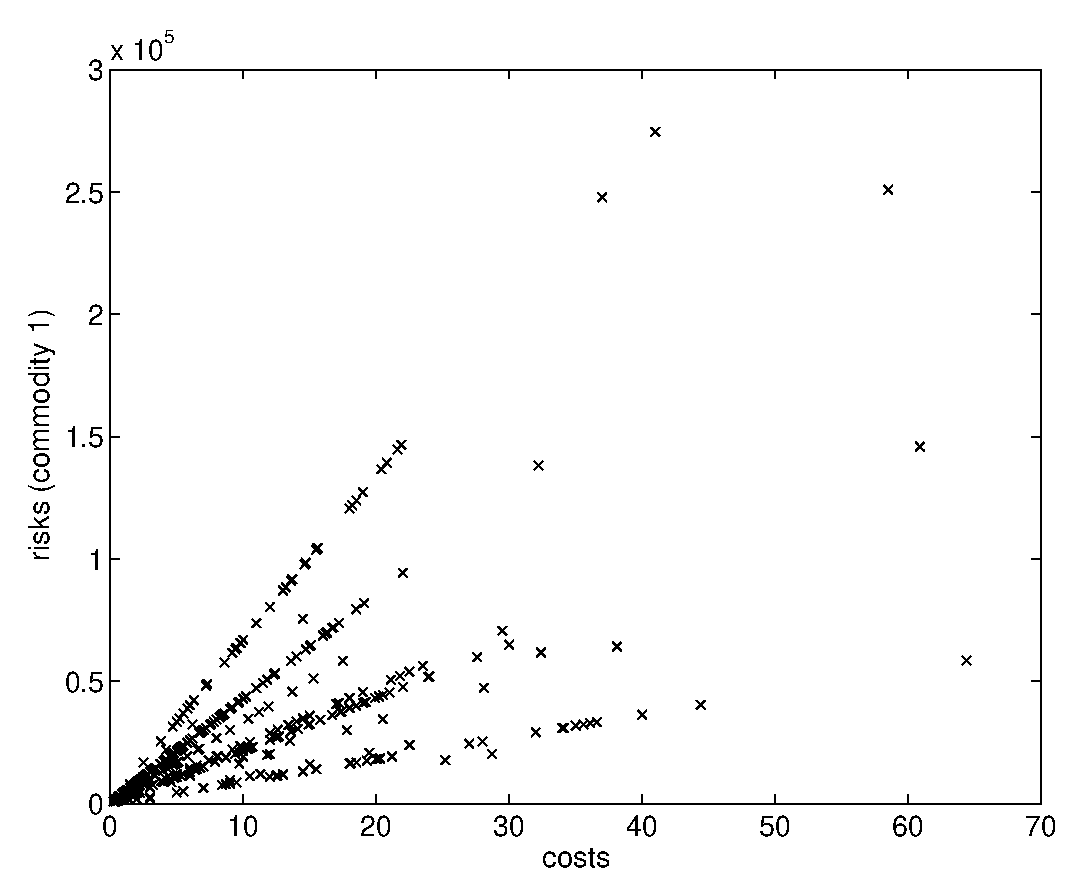
\includegraphics[width=0.48\columnwidth]{figs/correlationLazio41.eps}
	\hfill
	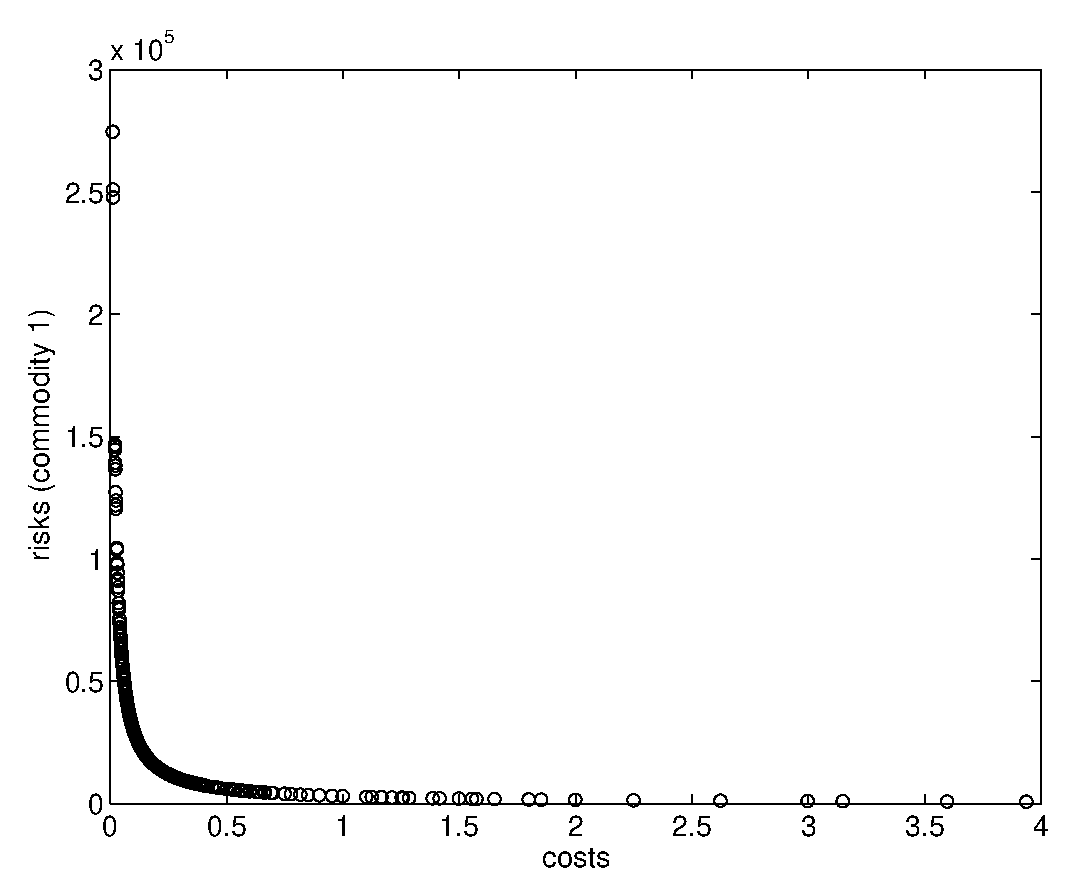
\includegraphics[width=0.48\columnwidth]{figs/correlationUncorrelated4.eps}
	\caption{\label{fig:correlation} Correlation between the costs and the risks of the first commodity for both the lazio\_4\_1 instance (left) and the uncorrelated\_4 instance (right). A single point corresponds to a single arc.}
\end{figure}

%We concentrated our analysis on a real-world case study \citep{bcg2009a}. We considered the road network of the Lazio region (located in the middle of Italy), and, in particular, its main transport roads. The network is composed of 311 nodes and 441 links. The risks $r_{ij}^c$ for each arc $(i,j) \in A$ and commodity $c \in C$ are evaluated as the societal risk computed as the number of people living inside the exposure zone around link $(i,j)$ (whose size depends on the hazmat type $c$ times the accident probability involving the vehicle), for details see  \citep{bcg2009a}. We considered from 2 to 10 origin-destination pairs on the network, each one associated with a number of commodities ranging from 1 to 3, for an overall number of shipments (commodities) between 2 and 30 (we recall that in our model each commodity is associated with one origin-destination pair). With each one of the latter scenarios we associated 10 instances; each instance has been generated by assigning uniformly at random a demand from 100 to 1000 tons to each shipment.

\subsection{Experimental Settings}
Except otherwise stated, we used the following parameter setting. We perform 10 independent runs of HypE for 2000 generations with a population size of 50, i.e., each algorithm run has a budget of 100,000 function evaluations. The reference point for the hypervolume indicator was chosen as $(10^8, 10^8, 10^8)$ for the instances with 2 and 3 commodities and as $(10^9, 10^9, 10^9)$ for all instances with 4 commodities. The reference point has been chosen according to the objective function values of the random initial populations, such that all initial solutions have a positive contribution to the hypervolume indicator. Note that the reason for using the same values in all objectives is the used PISA implementation of HypE. In all cases, the hypervolume computation is exact.

In terms of performance assessment, we present both visual comparisons of the final populations as well as statistical results. For the statistical results, the hypervolume indicator was also used as quality measure of the final populations as it is the only known unary quality indicator  which is a refinement of the Pareto dominance relation and therefore has important theoretical properties: whenever a set of solutions dominates another set, also the hypervolume value is higher; on the contrary, if the hypervolume indicator value of a set A is worse than for set B, we know that B cannot dominate A \citep{ztlf2003a,ztb2010a}. In order to compare algorithms with respect to their hypervolume indicator values, we use both box plots\footnote{As implemented in MATLAB R2008b.} and the Wilcoxon rank sum test\footnote{As implemented in the statistical programming language R, version 2.1.3.0.}.


\subsection{Differences Between Instances}
The basis for our experiments are 5 instances of the lazio network with 2 (lazio\_2), 3 (lazio\_3), and 4 commodities (lazio\_4\_1, lazio\_4\_2, and lazio\_4\_3) which differ also in the number of trucks for the commodities. Whereas the number of trucks for lazio\_3 and lazio\_4\_1 have been chosen randomly, lazio\_2 has the same number of trucks than the lazio\_3 instance for the first two commodities. The lazio\_4\_2 instance has only 1 truck more for commodity 4 than lazio\_4\_1 and overall three times the number of trucks for each commodity than the instance lazio\_4\_3, cp.\ Table~\ref{tab:instances}.

Figure~\ref{fig:compareAll} shows the non-dominated solutions of 10 independent HypE runs for each instance. What can be observed are three main statements. First of all, cost and risks of the found non-dominated solutions are highly correlated, as they are for each single arc in the problem formulations; therefore, the problem is not truly three-objective but rather bi-objective. Secondly, the range of the objective function values for the found non-dominated solutions follow the number of trucks in the problem instance, i.e., the more trucks a problem instance has the more costs, total and equity risk can be expected in the solutions found. However and thirdly, this relationship is not linear in the plots of Fig.~\ref{fig:compareAll} as can be seen, for example, between the lazio\_4\_2 and the lazio\_4\_3 instance. Though the number of trucks per commodity differs by a factor of 3 between them, the objective function values of the resulting non-dominated solutions after 2,000 generations are slightly further away. The reason for that is the much smaller search space for the lazio\_4\_3 instance which can be searched more exhaustively by the algorithm with the same number of function evaluations---resulting in a better convergence towards the Pareto front.

\begin{figure}
	\centering
	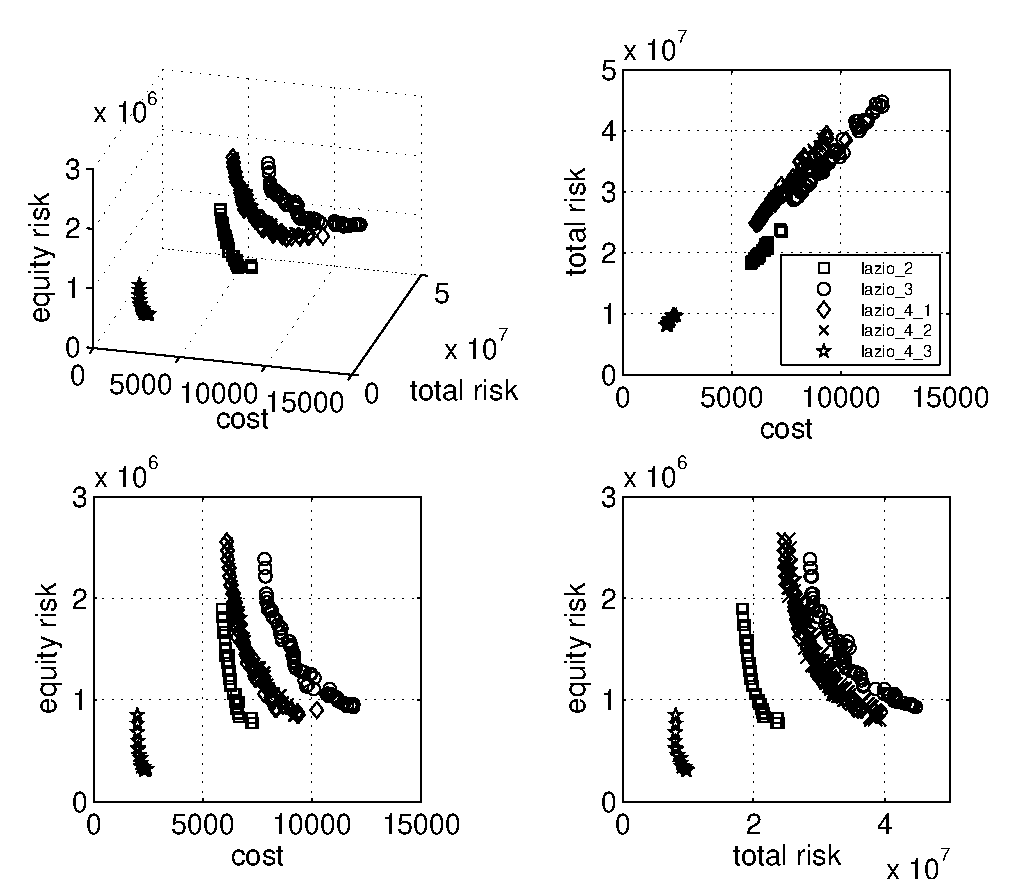
\includegraphics[width=0.75\columnwidth]{../experiments/randVsCost/compAll_2000gens.eps}
	\caption{\label{fig:compareAll} Comparison between the different instances lazio\_2 (squares), lazio\_3 (circles), lazio\_4\_1 (diamonds), lazio\_4\_2 (crosses), and lazio\_4\_3 (stars). Shown are the non-dominated solutions in the final populations of 10 independent HypE runs with population size 50 after 2000 generations.}
\end{figure}


\subsection{Convergence Towards the Pareto Front}
Figure~\ref{fig:hypervolumeOverTime} shows the boxplots of the hypervolume values for HypE with population size 50 and 100 for different number of generations. What can be seen is that, in general, the hypervolume indicator is maximized over time and that for the algorithm with population size 50, the hypervolume value starts to stagnate starting from around generation 1500 with the mean still going up but the variance staying high. The fact that all runs found a similar hypervolume value which is significantly higher than the one of the random population in the beginning (around $9.62\cdot 10^{26}$ for both algorithms) indicates that the algorithm found solution sets which are close to the Pareto front.


\begin{figure}
	\centering
	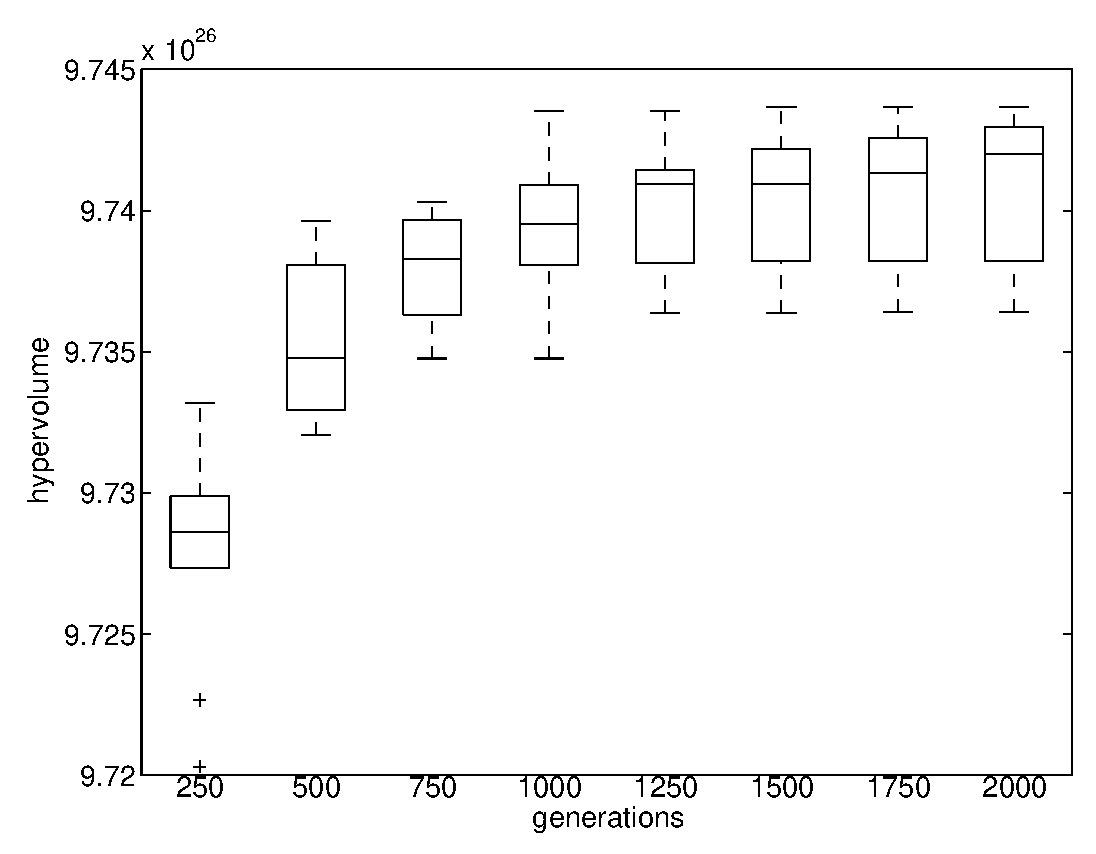
\includegraphics[width=0.48\columnwidth]{../experiments/randVsCost/hypervolumes/hypervolumeOverTime_50.eps}
	\hfill
	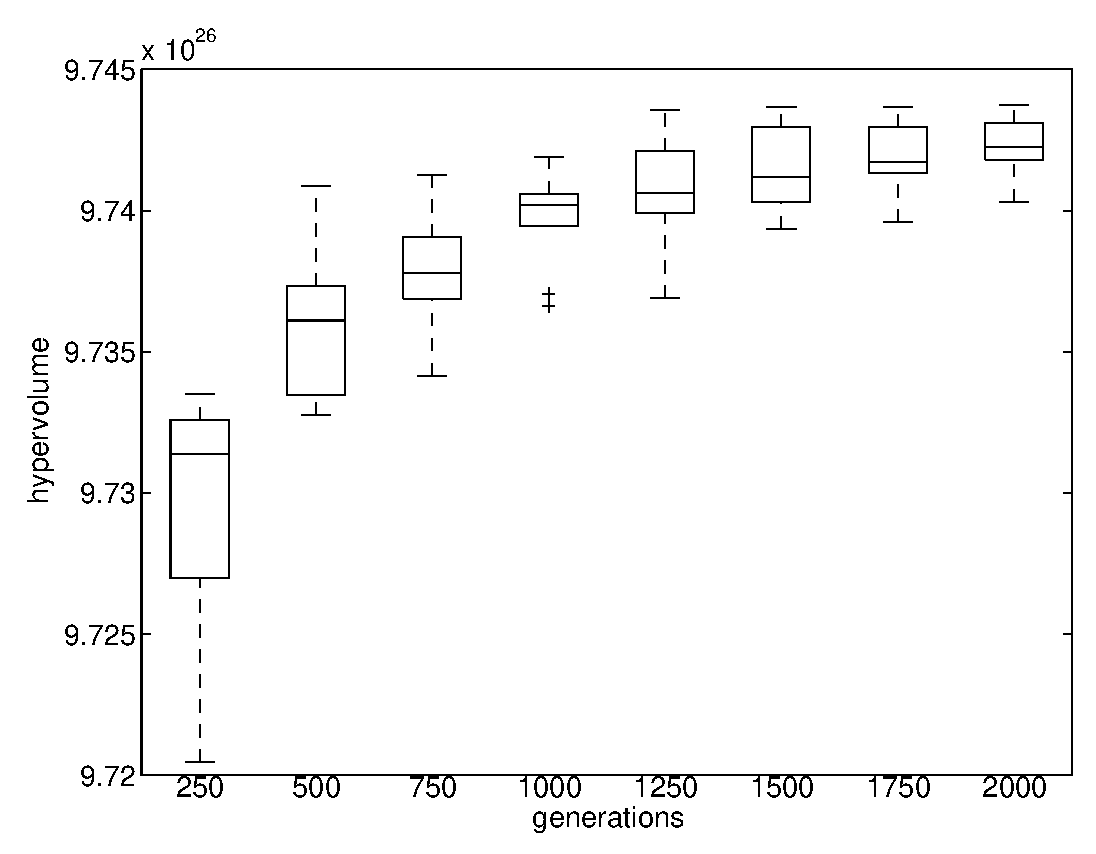
\includegraphics[width=0.48\columnwidth]{../experiments/randVsCost/hypervolumes/hypervolumeOverTime_100.eps}
	\caption{\label{fig:hypervolumeOverTime} Boxplots of hypervolume values over time for numbers of generations in $[250, \ldots, 2000]$ for HypE with population size 50 (left) and population size 100 (right) on the lazio\_4 instance.}
\end{figure}

\subsection{Random Initialization Versus Cost-Optimal Initialization}
In order to see the impact of the two different initialization schemes \emph{random} and \emph{cost-optimal}, we performed 10 runs of HypE with both initialization schemes for 2,000 generations and a population size of 50 as above. Figure~\ref{fig:randVsCostOriginal} shows the resulting non-dominated solutions of the final populations. Surprisingly, the cost-optimal initialization could not produce other solutions than the cost-optimal one itself. As we will see below, the reason is a high correlation between the risk and costs of each arc, which seemingly results in the fact that no non-dominated solution can be reached from the initial solution by the applied mutation operator. However, the comparison between the two initialization schemes on the lazio\_4\_1 instance shows that also the algorithm employing the random initialization can find solutions which are close to the Pareto front---improving over the hypervolume of the single cost-optimal solution in later generations, see the left-hand plot of Fig.~\ref{fig:costVsRandBoxPlots}. 

To show that the cost-optimal initialization is not useless, we run the algorithms again on the instance uncorrelated\_4 where the cost and risk values are fully uncorrelated. In this case, there are more local changes of the truck paths that result in non-dominated solutions and eventually in a larger variety of solutions found by the algorithm employing the cost-optimal initialization (see Fig.~\ref{fig:randVsCostNew}). Due to the fact that the cost-optimal initialization starts already on the Pareto-front, it also results in higher hypervolume values than for the random initialization variant---both for a low and a high number of generations, see the right-hand side plot of Fig.~\ref{fig:costVsRandBoxPlots}. All algorithms of Fig.~\ref{fig:costVsRandBoxPlots} are pairwisely significantly different with respect to their hypervolume values according to Wilcoxon rank sum tests with p-values below 0.01.


\begin{figure}
	\centering
	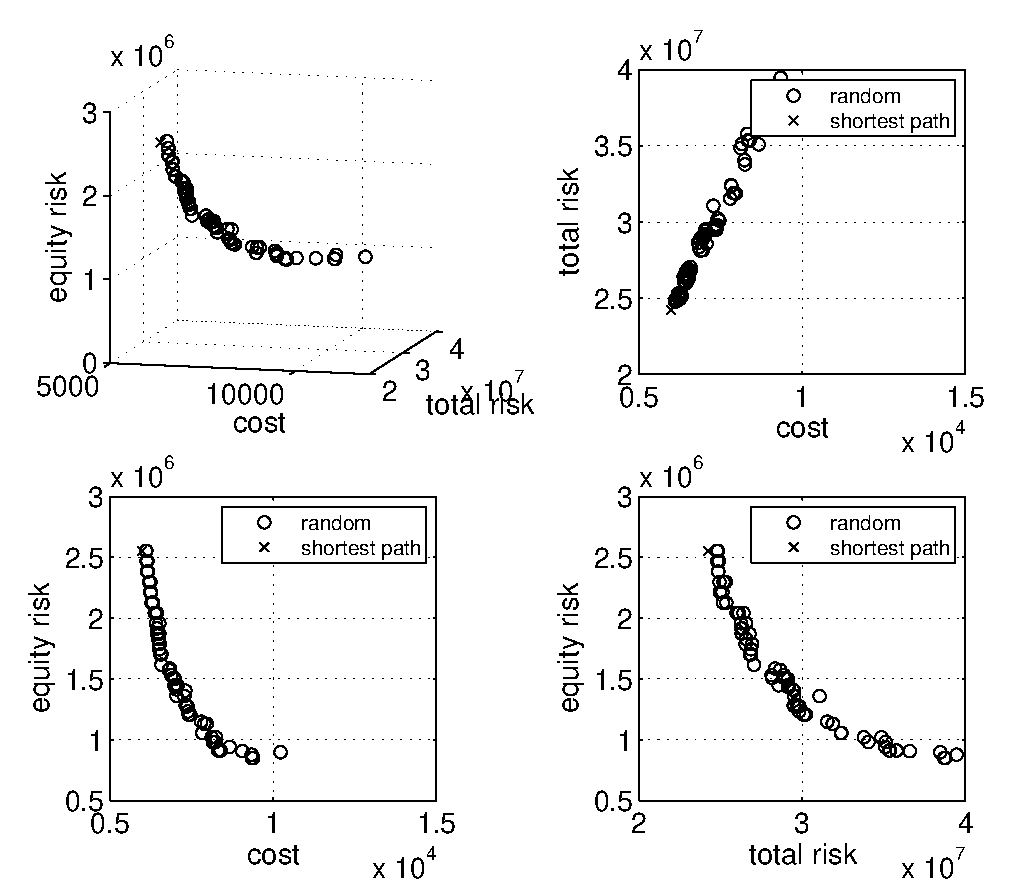
\includegraphics[width=0.75\columnwidth]{../experiments/randVsCost/randVsCost_ns4_1_OriginalCost_2000gens.eps}
	\vspace{-1em}
	\caption{\label{fig:randVsCostOriginal} Comparison between the random initialization ($\circ$) and the cost-optimal one ($\times$). Shown are the non-dominated solutions in the final populations of 10 independent HypE runs with population size 50 after 2000 generations for all three objectives (top left) and each combination of two objectives on the lazio\_4\_1 instance.}
\end{figure}

\begin{figure}
	\centering
	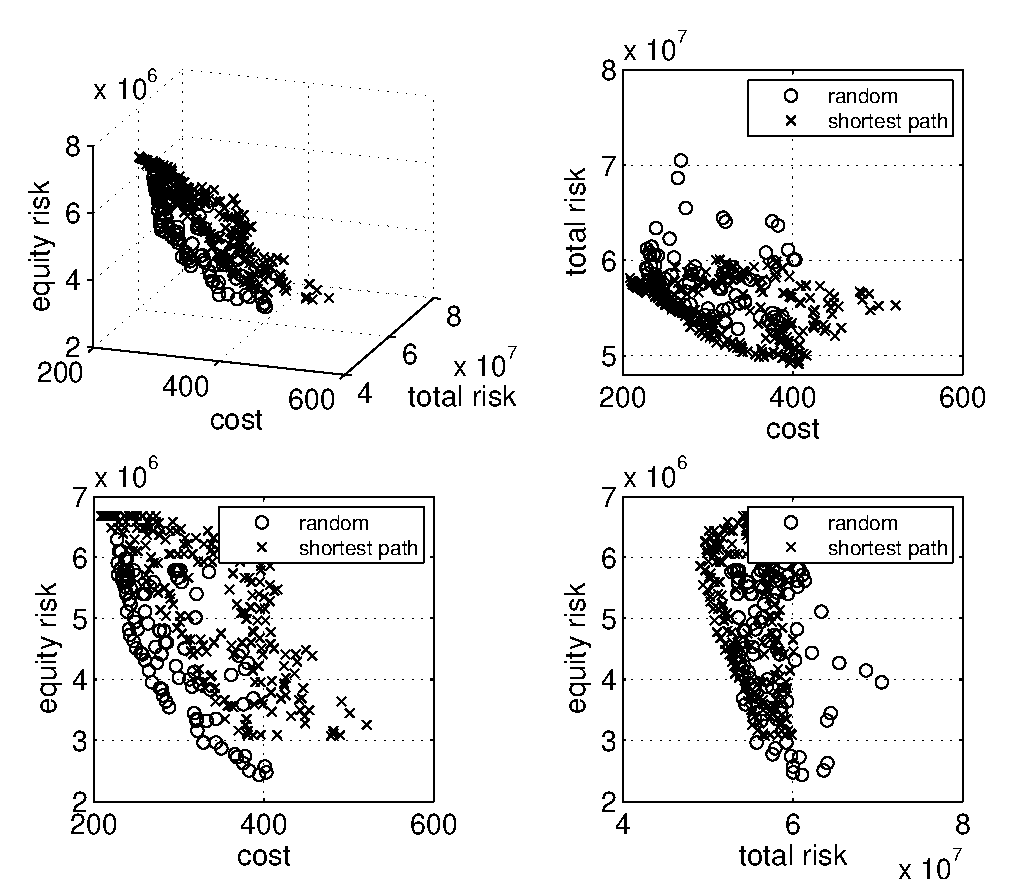
\includegraphics[width=0.75\columnwidth]{../experiments/randVsCost/randVsCost_ns4_1_New_2000gens.eps}
	\vspace{-1em}
	\caption{\label{fig:randVsCostNew} Comparison between the random initialization ($\circ$) and the cost-optimal one ($\times$). Shown are the non-dominated solutions in the final populations of 10 independent HypE runs with population size 50 after 2000 generations on the uncorrelated\_4 instance.}
\end{figure}


\begin{figure}
	\centering
	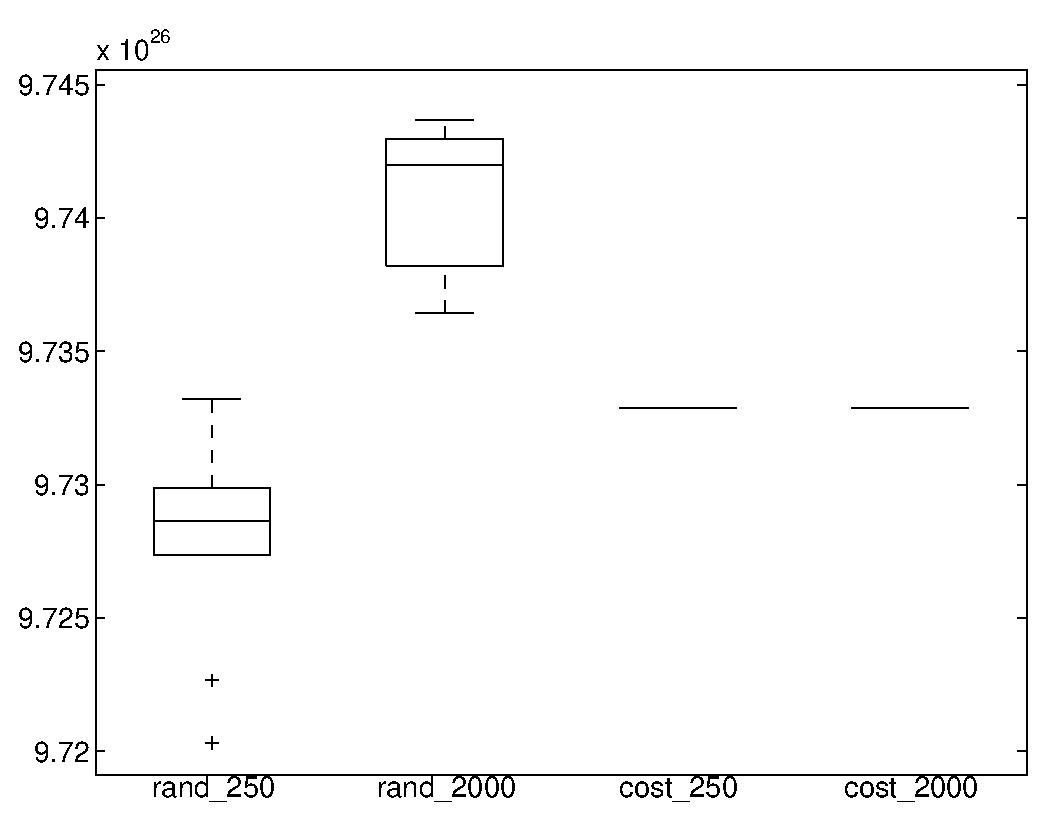
\includegraphics[width=0.48\columnwidth]{../experiments/randVsCost/hypervolumes/initBoxPlots_OriginalCosts.eps}
	\hfill
	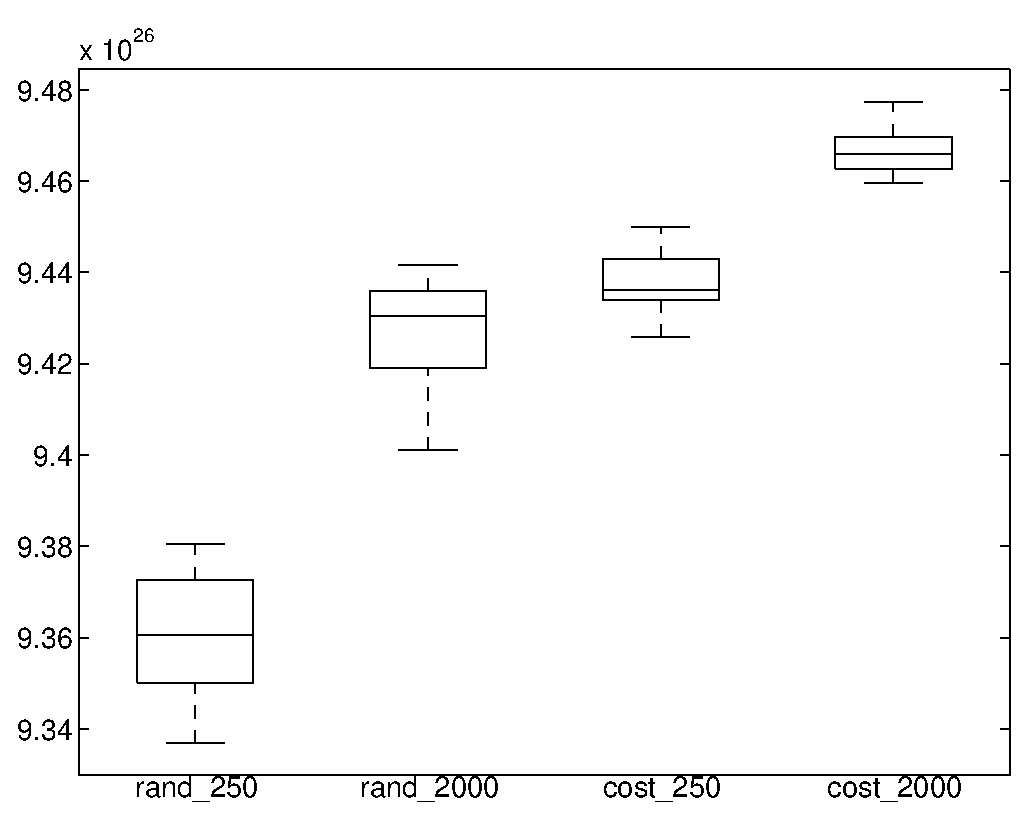
\includegraphics[width=0.48\columnwidth]{../experiments/randVsCost/hypervolumes/initBoxPlots_New.eps}
	\vspace{-1em}
	\caption{\label{fig:costVsRandBoxPlots} Comparison between the random initialization and the cost-optimal one.
	Shown are boxplots of hypervolume values for HypE with population size 50 on the lazio\_4 instance (left) and on the uncorrelated\_4 instance (right) after both 250 and 2000 generations.}
\end{figure}


\subsection{Changing the Population Size}
In the next experiment, we aim at showing that changing the population size of the algorithm in standard ranges does not change the algorithm outcome drastically. To this end, Fig.~\ref{fig:popsizes} shows the nondominated solutions of 10 independent runs after 100,000 function evaluations for three different versions of HypE where the population size changes from 50 over 100 to 200 on the largest instance lazio\_4\_1 with 4 commodities. From the visual inspection of the resulting solutions, we cannot make a statement about which population size to favor. When comparing the hypervolume values of the resulting populations, however, an effect is visible. Figure~\ref{fig:algoComparison} shows the corresponding box plots of the hypervolume values and one-sided Wilcoxon rank sum tests on the populations' hypervolume indicator values reveal statistical significant differences between two of the three possible algorithm pairs. With a $p$-value of $0.02163$, the null hypothesis of no differences between a population size of 50 and a population size of 100 has to be rejected in favor of stating that the algorithm variant with population size 50 is superior to the one with population size 100. For the comparison between population size 50 and population size 200, the $p$-value equals $0.0144$ with the population size 50 being better whereas the comparison between population size 100 and population size 200 does not reveal a statistical difference (the $p$-values of the one-sided Wilcoxon tests are $0.2179$ and $0.8035$ respectively). 

Although these results indicate that smaller population sizes might be always favorable, this is not the case as additional experiments with a population size of 25 show (see the box plot in Fig.~\ref{fig:algoComparison}). The Wilcoxon rank sum test comparing population sizes 25 and 50 results in a $p$-value of $0.004465$ whereas the other comparisons are not statistically significantly different. To conclude, among the tested population sizes, 50 seems to be the best choice for budgets around 100,000 function evaluations but the population size is not a parameter that is difficult to adjust for the user. According to the runtime of the algorithm, we recommend to keep the population size of the algorithm around 50 as the HypE implementation in PISA becomes too costly if the population size is much larger. Ten runs with 2000 iterations and population size 200, for example, need already around 20 hours to complete on an Intel Core2 Duo with 2.8GHz.

\begin{figure}%
	\centering
	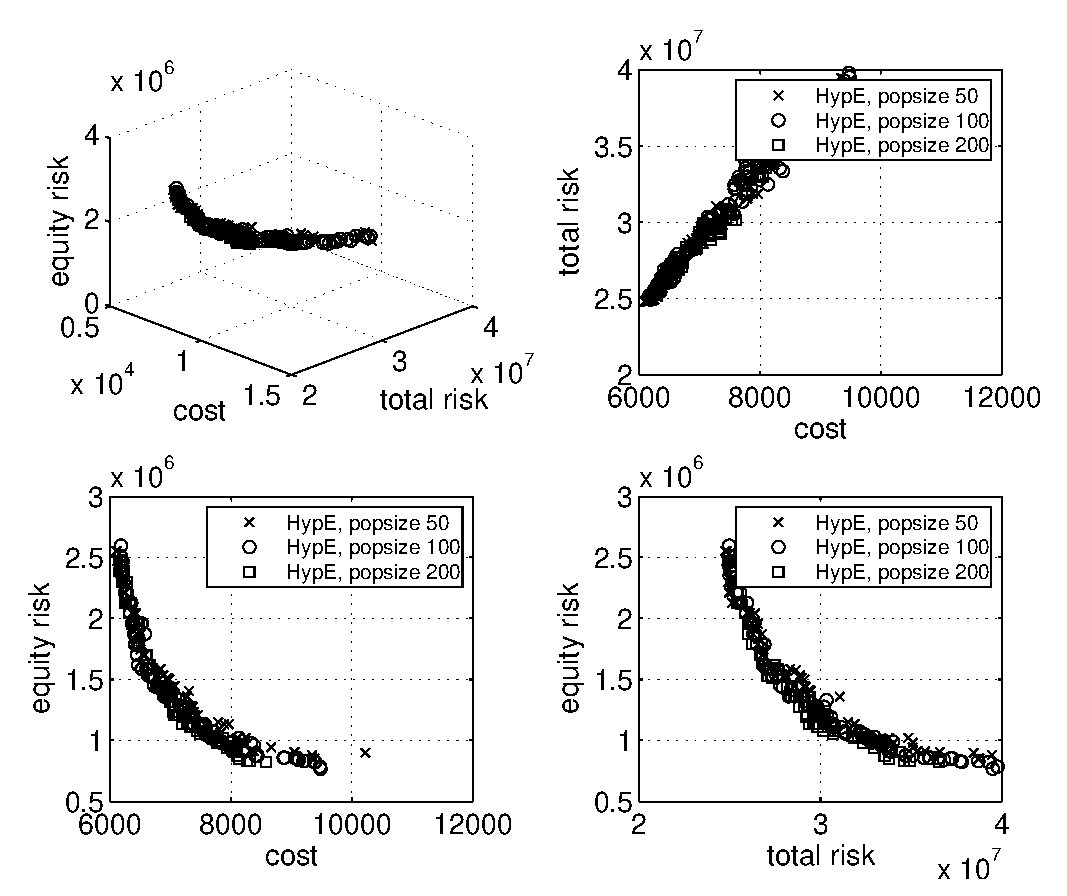
\includegraphics[width=0.75\columnwidth]{../experiments/randVsCost/diffPopsizes}%
	\vspace{-1em}
	\caption{\label{fig:popsizes} Nondominated solutions of 10 independent runs after 100,000 function evaluations for HypE with a population size of 50 ($\times$), 100 ($\circ$), and 200 ($\square$) respectively.}
\end{figure}

\begin{figure}%
	\centering
	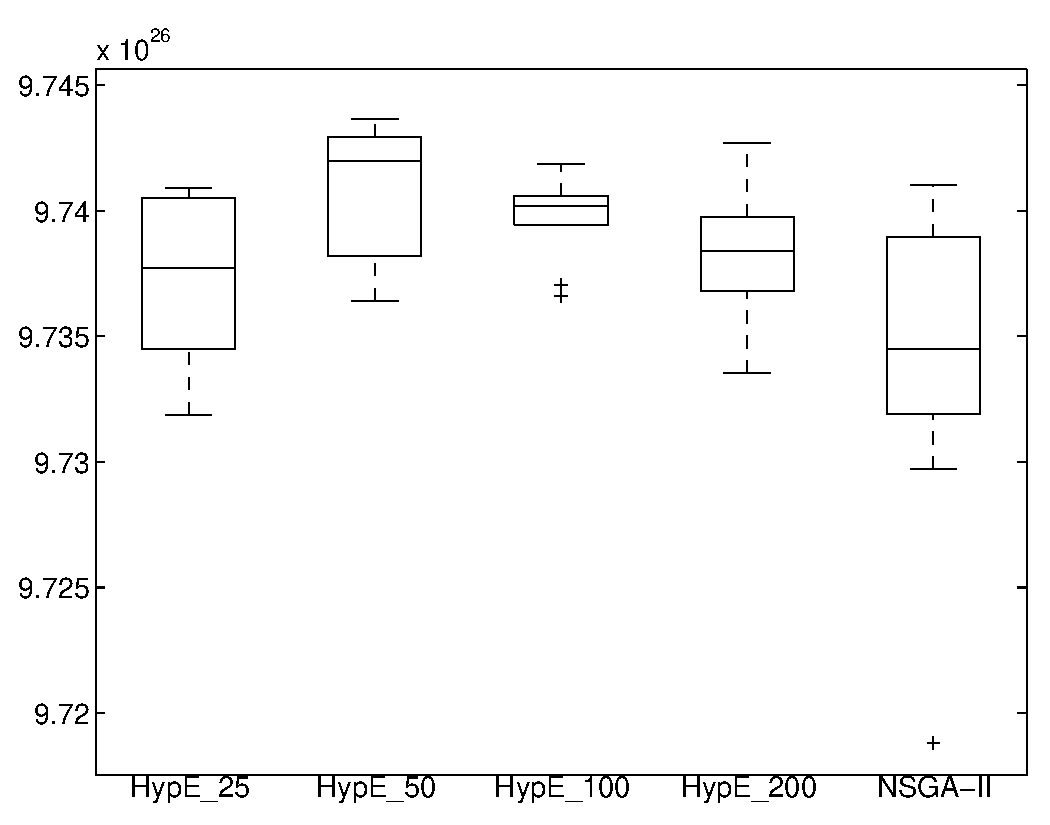
\includegraphics[width=0.5\columnwidth]{../experiments/randVsCost/hypervolumes/algoComparison}%
	\caption{\label{fig:algoComparison} Boxplots of the hypervolume values of 10 independent runs after 100,000 function evaluations of HypE with a population size of 25, 50, 100, and 200, as well as for NSGA-II.}
\end{figure}

\subsection{Changing the Environmental Selection}
With a last experiment, we show the influence of the algorithm's environmental selection scheme on the performance and in particular how this can be used to steer the search towards specific regions of the Pareto front.

Instead of the environmental selection of HypE \citep{bz2011a}, other selection schemes can be easily used with the PISA framework and we show the results of two other algorithms exemplary. On the one hand, we employ the famous NSGA-II selection scheme \citep{dapm2002a} and, on the other hand, we use a generalized version of HypE towards a generalized weighted hypervolume indicator \citep{abbz2009b,bbtz2011a}. The boxplots of the resulting hypervolume indicator values after 100,000 function evaluations (population of size 100 after 1000 generations for NSGA-II and population size of 25 and 4,000 generations for W-HypE) are shown in Fig.~\ref{fig:algoComparison}. What can be seen is that both algorithms show a reduced performance regarding the standard hypervolume value, with W-HypE being much worse than NSGA-II. For NSGA-II, this decrease  in hypervolume is expected as its environmental selection schemes does not optimize the hypervolume indicator directly as HypE does. Moreover, NSGA-II is known to become less effective than in bi-objective problems when the number of objectives increases \citep{wbn2007a,bz2011a}. This is less the case for indicator-based algorithms such as HypE which were specifically proposed to circumvent the problems of algorithms optimizing quality measures that do not comply with the Pareto dominance relation such as the crowding distance of NSGA-II.

The reason for the reduced performance in the standard hypervolume indicator for W-HypE, on the other hand, can be explained in a different way. W-HypE and the underlying weighted hypervolume indicator was developed to steer the search towards regions of the objective space that have been specified by the user. To this end, instead of the standard hypervolume indicator, the weighted hypervolume indicator of \citep{zbt2007a} is optimized in W-Hype \citep{abbz2009b,bbtz2001a}. The idea behind W-HypE is that solutions in objective space regions with a higher weight will get a higher fitness due to the \emph{weighted} hypervolume they dominate. Furthermore, in order to be efficient also for a large number of objectives, W-HypE does not calculate the weighted hypervolume indicator values exactly but instead samples them. Here, 10,000 samples are used in each iteration of the algorithm. For details on the algorithm, we refer to the original publication \citep{bz2011a}.

To show the principles of W-HypE in the application of our hazmat routing problem, we defined the weight of W-HypE's underlying weighted hypervolume indicator as constant in a box with corners $[7\cdot 10^3, 3\cdot 10^7, 5\cdot 10^5]$ and $[10^4, 4\cdot 10^7, 1.1\cdot 10^6]$ and zero otherwise. Instead of optimizing the standard hypervolume indicator as HypE does, W-HypE now optimizes this weighted hypervolume indicator as a secondary selection criterion after employing a non-dominated sorting. As a result, it is finding better, i.e., dominating solutions in regions in or close to the box. Figure~\ref{fig:whype} shows the resulting non-dominated solutions of both algorithms W-HypE and HypE with population size 25 after 10 independent runs of 4,000 generations together with the sampling box. While HypE originally finds 6 non-dominated solutions within the box, W-HypE finds 14 within the same budget of function evaluations. When both algorithm outcomes are combined, it turns out that 13 of W-HypE's solutions within the box are still non-dominated while 5 out of the 6 solutions found by HypE are dominated by W-HypE solutions. It has to be noted that the advantage of W-HypE over HypE within the pre-defined box can be observed both in early and late generations (results not shown here).


\begin{figure}
	\centering
	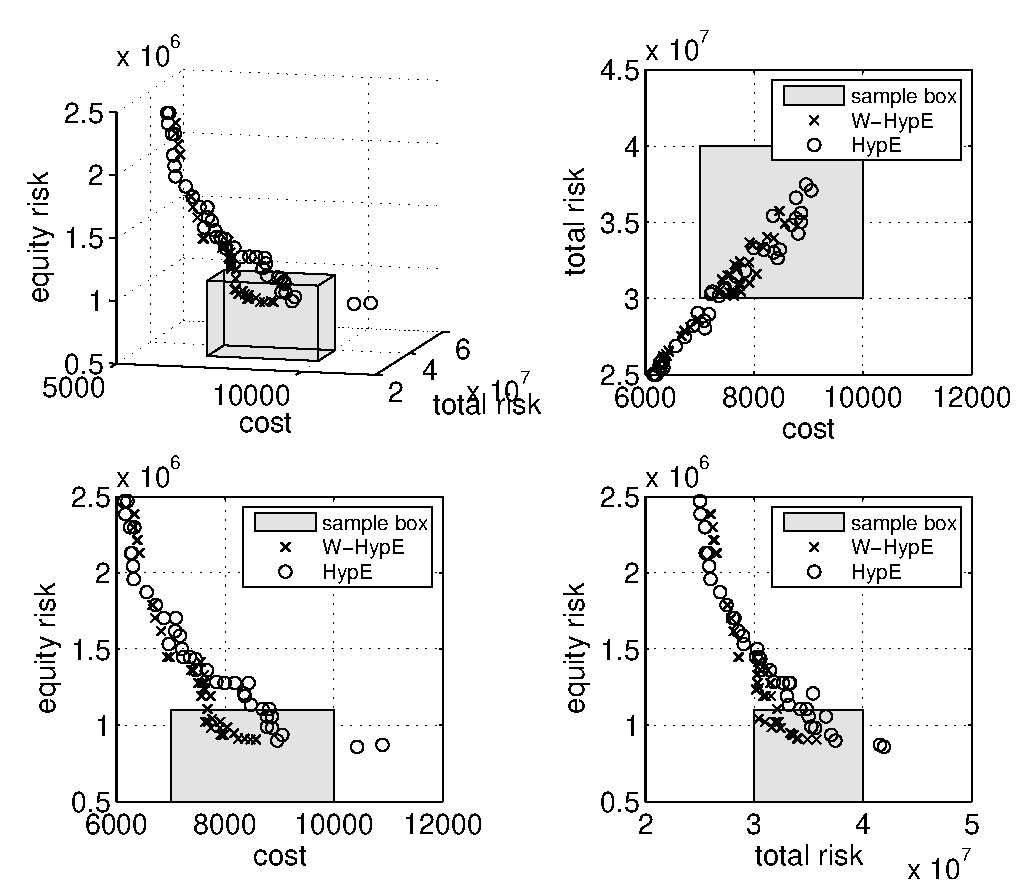
\includegraphics[width=0.75\columnwidth]{../experiments/randVsCost/WHypEVsHypE_ns4_1_OriginalCosts2.eps}
	\vspace{-1em}
	\caption{\label{fig:whype} Comparison between the standard HypE selection ($\circ$) with the one of W-HypE ($\times$) when the weighted hypervolume indicator is only sampled in the gray shaded box $[7\cdot 10^3, 10^4]\times[3\cdot 10^7, 4\cdot 10^7]\times[5\cdot 10^5, 1.1\cdot 10^6]$. Shown are all non-dominated solutions for each algorithm after 10 runs with 4,000 generations and population size 25.}
\end{figure}


\subsection{The Feasibility of the EMO Approach}
Due to their heuristic nature, evolutionary multiobjective optimization algorithms like the one presented in this study cannot guarantee that the solutions found are actually Pareto-optimal. However, as we have seen above, the proposed algorithm is able to produce a set of non-dominated solutions in reasonable time. In particular the comparison with the cost-optimal solution shows that the randomized algorithm can find solutions close to the Pareto front. The found sets of non-dominated solutions can be a starting point for a decision maker to investigate the trade-offs between the objectives and to decide in which objective space region interesting Pareto-optimal solutions should be searched for with more involved algorithms---be it exact algorithms or specialized evolutionary algorithms such as the mentioned W-HypE variant.

Regarding the two initialization schemes, it turns out that in combination with the (local and quite simple) variation operator, the cost-optimal initialization does not allow the algorithm to find additional solutions besides the initial one on the Lazio instances. However, if the cost and total risk objectives are uncorrelated, this cost-optimal initialization has advantages over the random initialization in all stages of the search when compared with respect to the hypervolume indicator. In general, however, we suggest to use the random initialization\footnote{or a combination with a more exploring mutation operator} if the costs and risks are highly correlated.

Using other initializations as well as additional variation operators from the literature is easily possible with the proposed algorithm but their investigation is left for future research. For example, one can think of a ``more random'' initialization where the initial truck paths are generated by iteratively applying the mutation operator on the empty path. Also the multiple application of the described mutation operator within one single mutation might be beneficial as the explored space of neighbored paths is larger in comparison to the current mutation. Well-designed crossover operators can also be expected to be beneficial to the problem when, for example, good sub-paths can be exchanged between solution pairs. 

Overall, it is to say that the approach is very general and can easily be adapted if the problem formulation is (slightly) changed as it is often the case in practice, e.g., if different numbers of trucks or different types of vehicles with different loads are available. Also in the case when the definition of total and equity risk changes, it is only the objective function code that needs to be changed---a big advantage of blackbox optimizers such as the proposed EMO algorithm.
	

%%%%%%%%%%%%%%%%%%%%%%%%%%%%%%%%%%%%%%%%%%%%%%%%%%%%%%%%%%%%%%%%%%%%%%%%%
\section{Conclusions} \label{S_FW}
%%%%%%%%%%%%%%%%%%%%%%%%%%%%%%%%%%%%%%%%%%%%%%%%%%%%%%%%%%%%%%%%%%%%%%%%%
The transportation of hazmats is an important optimization problem in the field of sustainable development and in particular the equitable distribution of risks is of high interest. Within this study, we formalize this transportation problem as the minimization of three objectives and propose to use an evolutionary multiobjective optimization (EMO) algorithm to cope with the non-linear equity risk objective in a true multiobjective sense.

The algorithm, based on the state-of-the-art environmental selection scheme of HypE, employs a problem-specific variable-length representation and a mutation operator which are known to be well-suited for shortest path problems from theoretical studies. With its random initialization, the algorithm allows to find sets of non-dominated solutions in reasonable time which are close to the Pareto-optimal front. For the tested real-world instances with the road network of the Lazio region and dozens of trucks for up to 4 hazmat commodities, the current Java implementation allows to finish the 100,000 function evaluations of a single experiment within less than 15 minutes on a standard Intel Core i5 laptop. In addition, the fact that EMO algorithms are \emph{anytime} algorithms is another advantage which allows the user to interrupt the algorithm at anytime while the algorithm provides a feasible set of solutions.

In future work, one might want to look further into adding (simple) heuristics within the EMO algorithm in order to improve the convergence of the algorithm. For example, one can observe that the solutions produced by the algorithm sometimes uses one and the same arc within a truck path, hence introducing cycles. With the three objectives cost, total and equity risk, such cycles can be easily prevented within the variation operator which might eventually result in a faster convergence of the algorithm to the Pareto front. Another path for future research is the consideration of more realistic problem instances. Stochastic risks or dynamically changing instances (for example due to road closures or traffic jams) would be interesting to address---challenges that have been dealt with by EMO algorithms in other application domains already before \cite{deb2001a,cvl2007a}.



\section{Acknowledgments}
The authors would like to thank Stefano Giordani for providing us with the instances of the Lazio network. Moreover, Dimo Brockhoff would like to acknowledge support from the CNRS-Microsoft chair \emph{Optimization for Sustainable Development} during his time at Ecole Polytechnique, Palaiseau, France.


% 
 \bibliographystyle{plainnat}
 \footnotesize
 \bibliography{all}






\end{document}

%%
%% End of file `elsarticle-template-1a-num.tex'.
